\documentclass{beamer}

\usetheme{CambridgeUS}
\usepackage{graphicx}
\usepackage{hyperref}

\title{Social Algorithms and Optimization}
\author{Jorge Aldair Cortés López}
\institute{Centro de Investigación en Computación}
\date{\today}

\begin{document}

\begin{frame}
    \titlepage
\end{frame}

\begin{frame}{Contenido}
    \tableofcontents
\end{frame}

\section{Referencias}

\begin{frame}{Referencias}
\begin{thebibliography}{30}
\bibitem{faridmehr2023mtbo}
I. Faridmehr, M.L. Nehdi, and I.F. Davoudkhani,
"Mountaineering team-based optimization: A novel human-based metaheuristic algorithm",
\textit{Mathematics}, vol. 11, no. 5, 2023.
Available at: \url{https://www.mdpi.com/2227-7390/11/5/1273}.

\bibitem{srinivasan2013social}
S. Srinivasan and S. Ramakrishnan,
"A social intelligent system for multi-objective optimization of classification rules using cultural algorithms",
\textit{Computing}, vol. 95, no. 1, pp. 21–45, 2013. 
Available at: \url{https://link.springer.com/article/10.1007/s00607-012-0246-4}.

\bibitem{6973911}Gong, Y., Zhang, J. \& Li, Y. From the social learning theory to a social learning algorithm for global optimization. {\em 2014 IEEE International Conference On Systems, Man, And Cybernetics (SMC)}. pp. 222-227 (2014)

\end{thebibliography}
\end{frame}

\begin{frame}{Referencias}
\begin{thebibliography}{30}
\bibitem{altay2019performance}
E.V. Altay and B. Alatas,
"Performance comparisons of socially inspired metaheuristic algorithms on unconstrained global optimization",
\textit{Proceedings of IC4S}, Springer, 2019. 
Available at: \url{https://link.springer.com/chapter/10.1007/978-981-13-0341-8_15}.

\bibitem{kulkarni2018socio}
M. Kumar, A.J. Kulkarni, and S.C. Satapathy,
"Socio evolution \& learning optimization algorithm: A socio-inspired optimization methodology",
\textit{Future Generation Computer Systems}, vol. 88, pp. 653–674, 2018.
Available at: \url{https://www.sciencedirect.com/science/article/pii/S0167739X17317259}.

\bibitem{maheri2021survey}
A. Maheri, S. Jalili, Y. Hosseinzadeh, and R. Khani,
"A comprehensive survey on cultural algorithms",
\textit{Swarm and Evolutionary Computation}, 2021. 
Available at: \url{https://www.sciencedirect.com/science/article/pii/S2210650221000079}.

\end{thebibliography}
\end{frame}


\begin{frame}{Referencias}
\begin{thebibliography}{30}

\bibitem{kumar2019socio}
M. Kumar and A.J. Kulkarni,
"Socio-inspired optimization metaheuristics: A review",
in \textit{Socio-cultural inspired metaheuristics}, Springer, 2019.
Available at: \url{https://link.springer.com/chapter/10.1007/978-981-13-6569-0_12}.

\bibitem{jalili2022cultural}
S. Jalili,
"Cultural Algorithms",
in \textit{Engineering Optimization: Methods and Applications}, Springer, 2022.
Available at: \url{https://link.springer.com/content/pdf/10.1007/978-981-19-4633-2.pdf}.

\bibitem{Neme2009}Neme, A. \& Hernández, S. Algorithms Inspired in Social Phenomena. {\em Nature-Inspired Algorithms For Optimisation}. pp. 369-387 (2009),  \url{https://doi.org/10.1007/978-3-642-00267-0_13}

\end{thebibliography}
\end{frame}


\section{Antecedentes}
\begin{frame}{Antecedentes}
    \begin{itemize}
        \item La evolución de los algoritmos bioinspirados (Nature-inspired algorithms) se corresponde con la evolución de los sistemas naturales.         
    \end{itemize}

    \vspace{0.5cm}
    \centering
    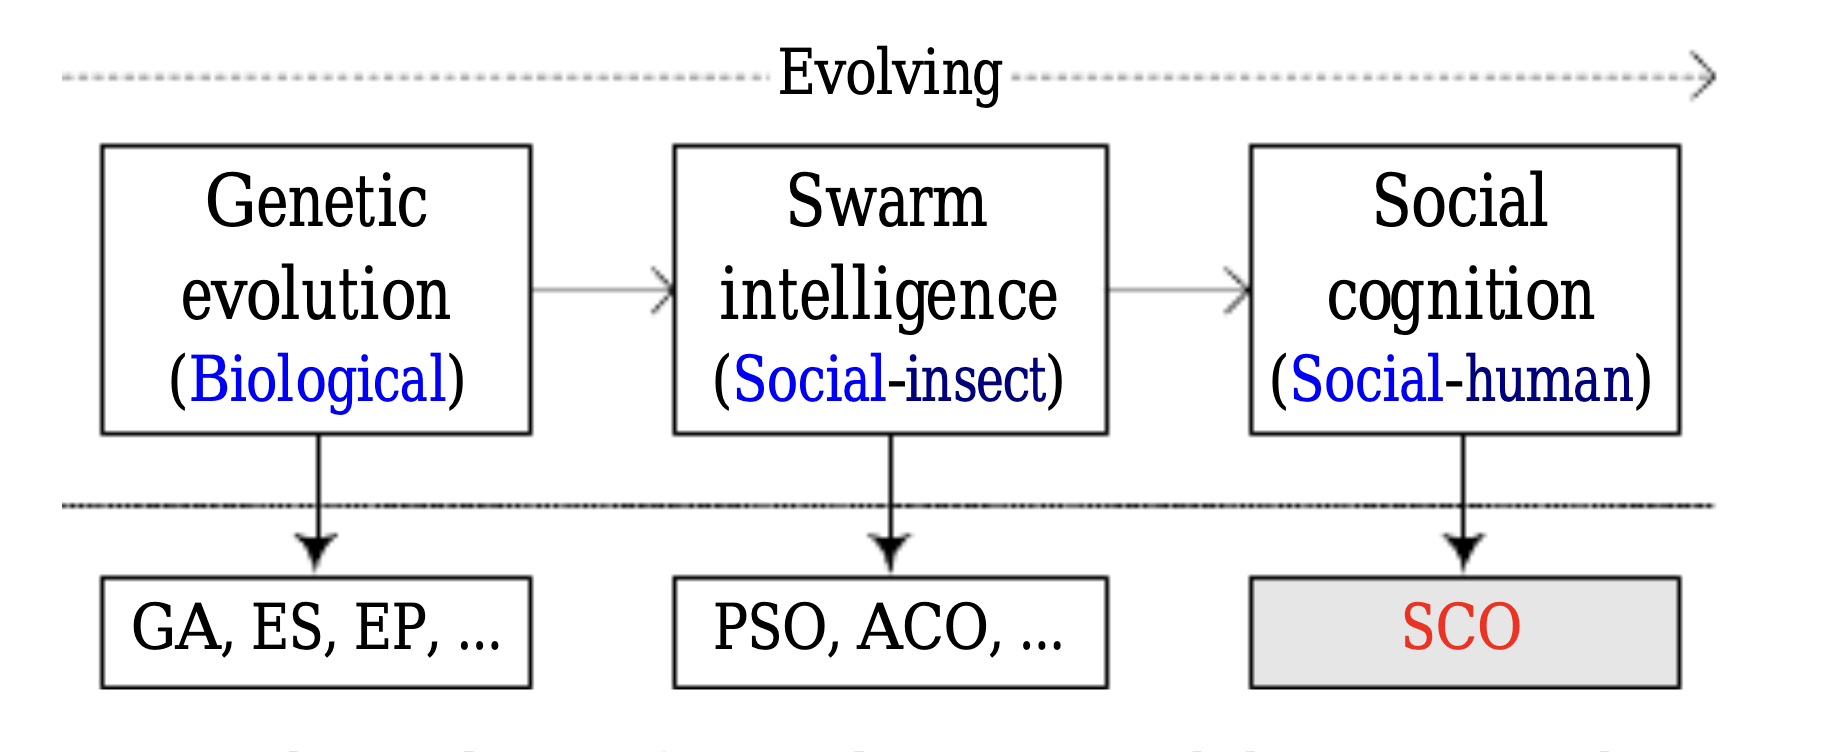
\includegraphics[width=0.9\textwidth]{classification_1.png}

\end{frame}

\begin{frame}{Antecedentes}
\begin{itemize}
    \item No solo los humanos tienen comportamiento sociales. Algunos algoritmos basados en enjambres, también utilizan principios sociales, cómo las hormigas, termitas y las arañas.
    \item Sin embargo, se prioriza el conocimiento desarrollado acerca de la inteligencia social, teniendo cómo principal antecedentes las interacciones sociales de los primates y de los humanos, pues se considera que éstas interacciones son \textit{más complejas}.
\end{itemize}
\end{frame}

\begin{frame}{Antecedentes}
    \begin{itemize}
        \item Se propone en la literatura, la siguiente clasificación de las metaheurísticas
    \end{itemize}
    \vspace{0.5cm}
    \centering
    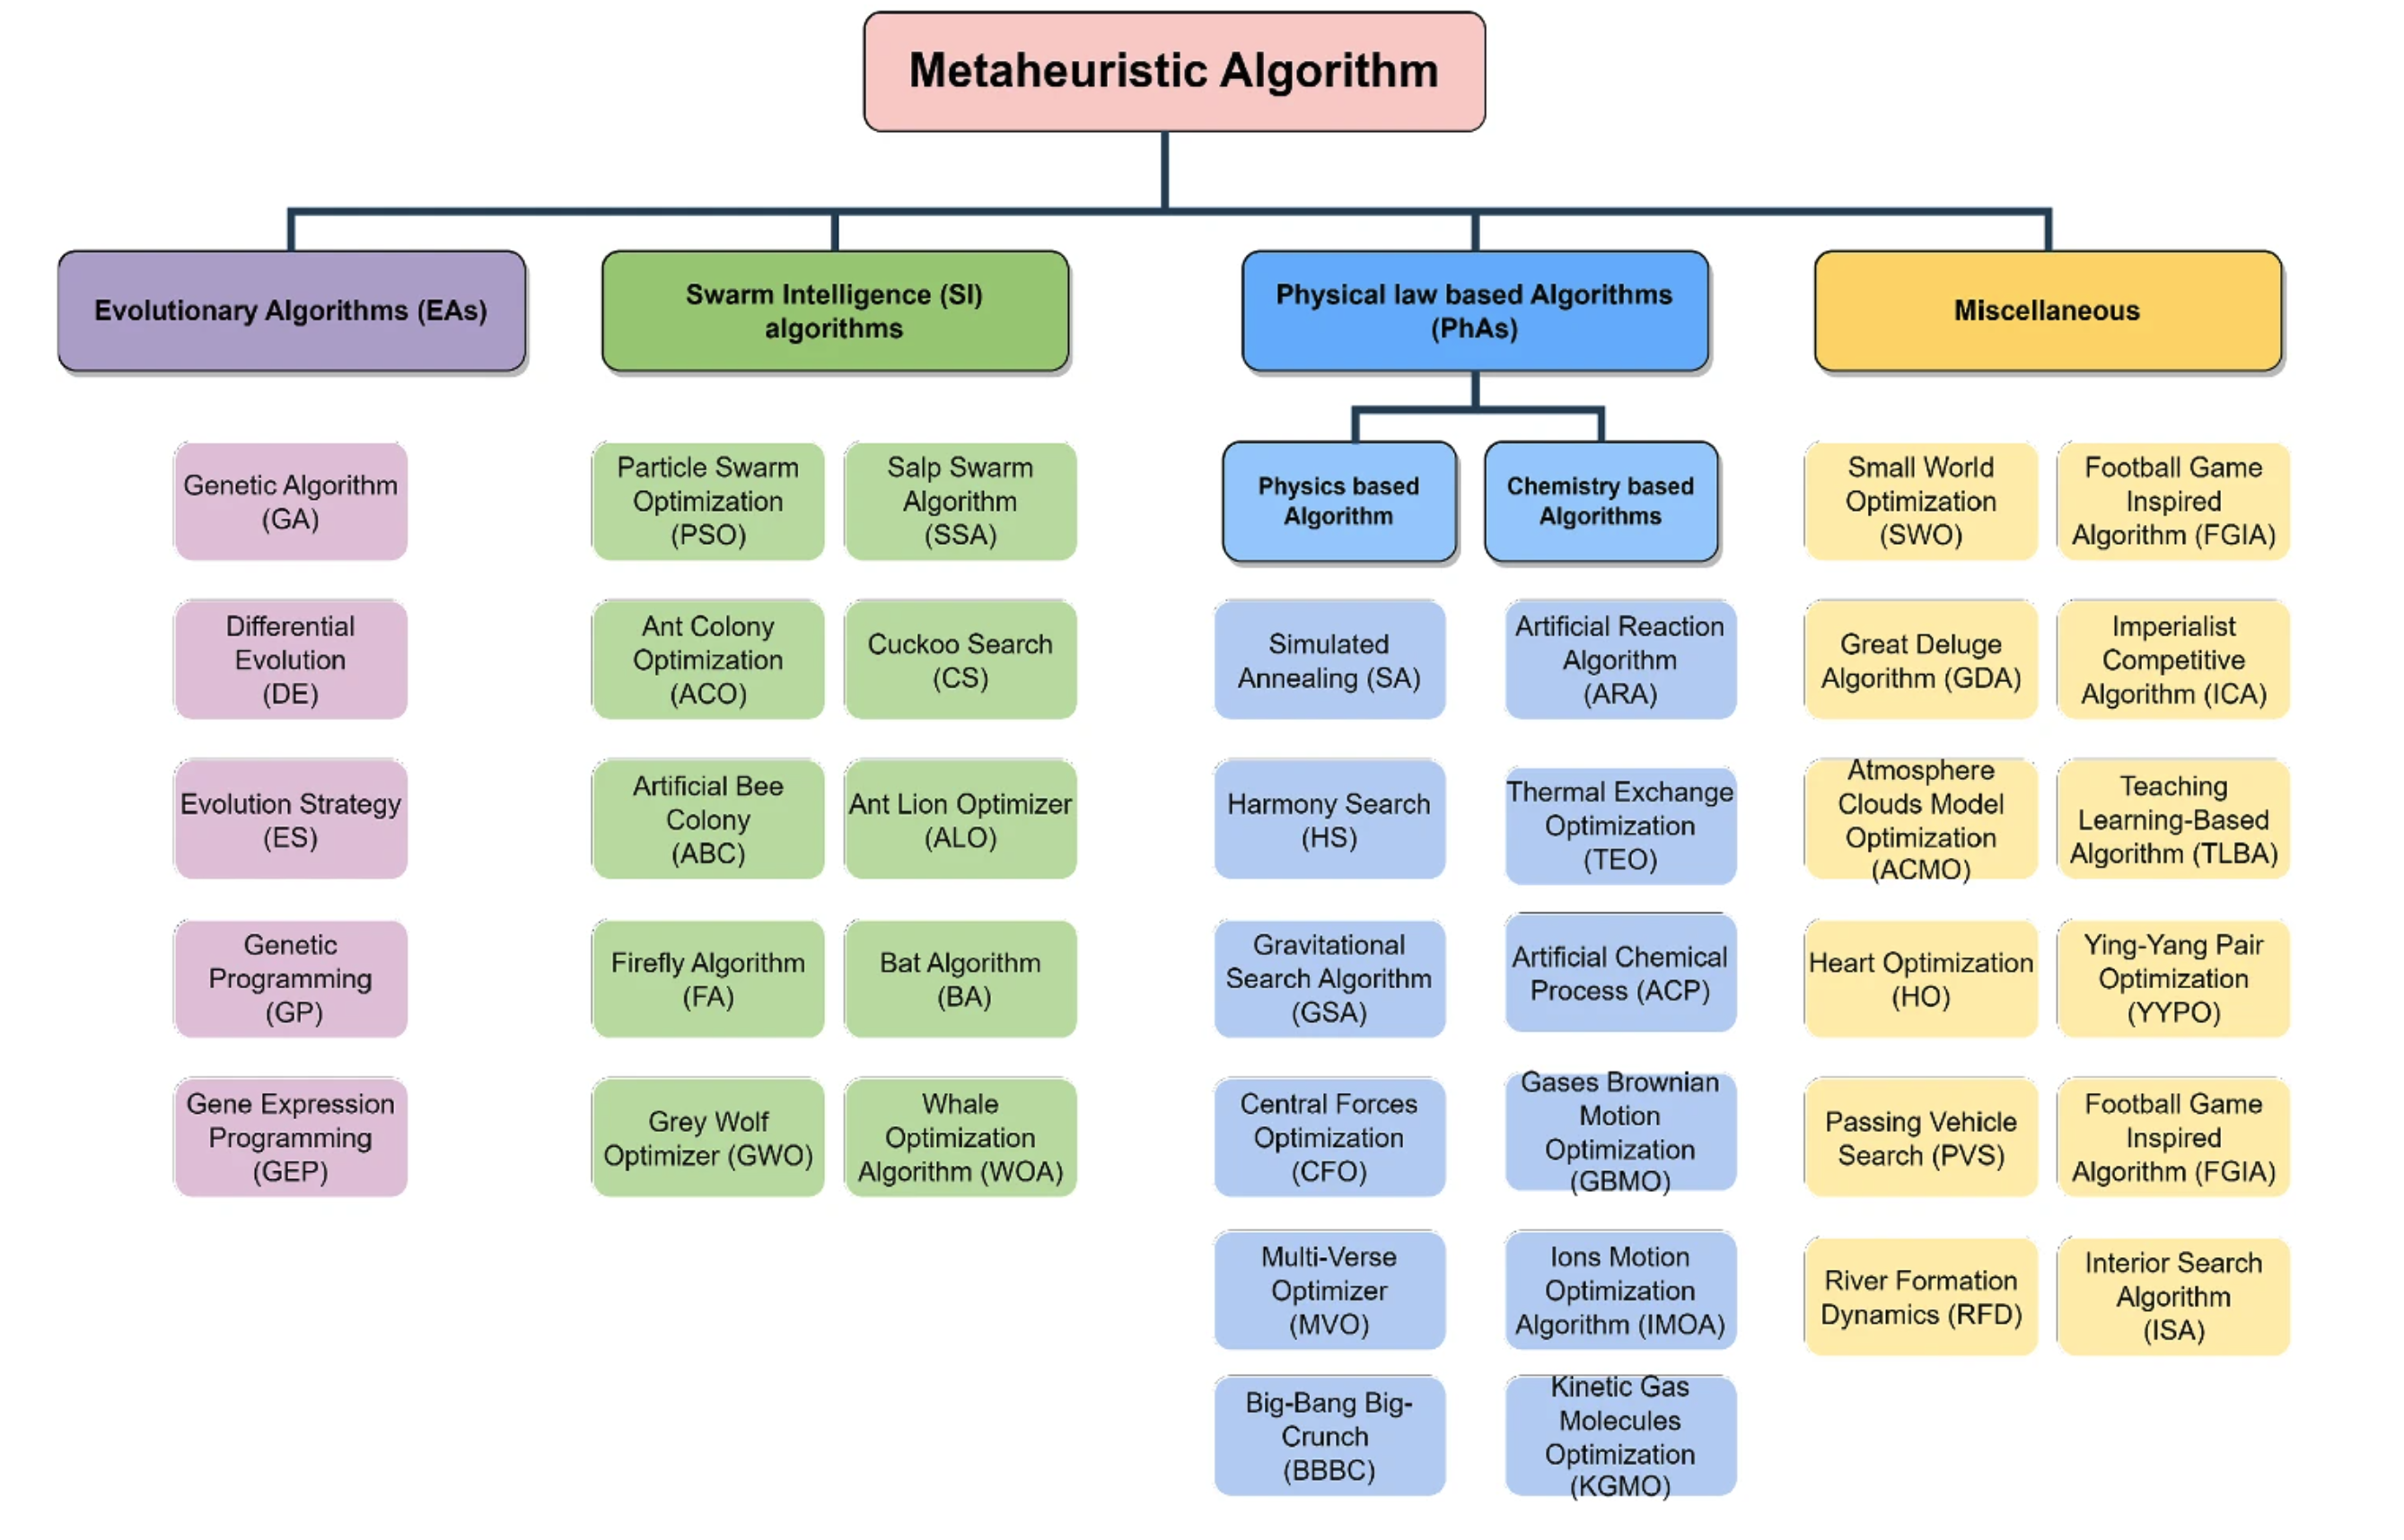
\includegraphics[width=0.9\textwidth]{mataheuristic-class.png}
\end{frame}

\begin{frame}{Antecedentes}
    \begin{itemize}
        \item Se propone en la literatura, la siguiente clasificación de los algoritmos bioinspirados  
    \end{itemize}
    \vspace{0.5cm}
    \centering
    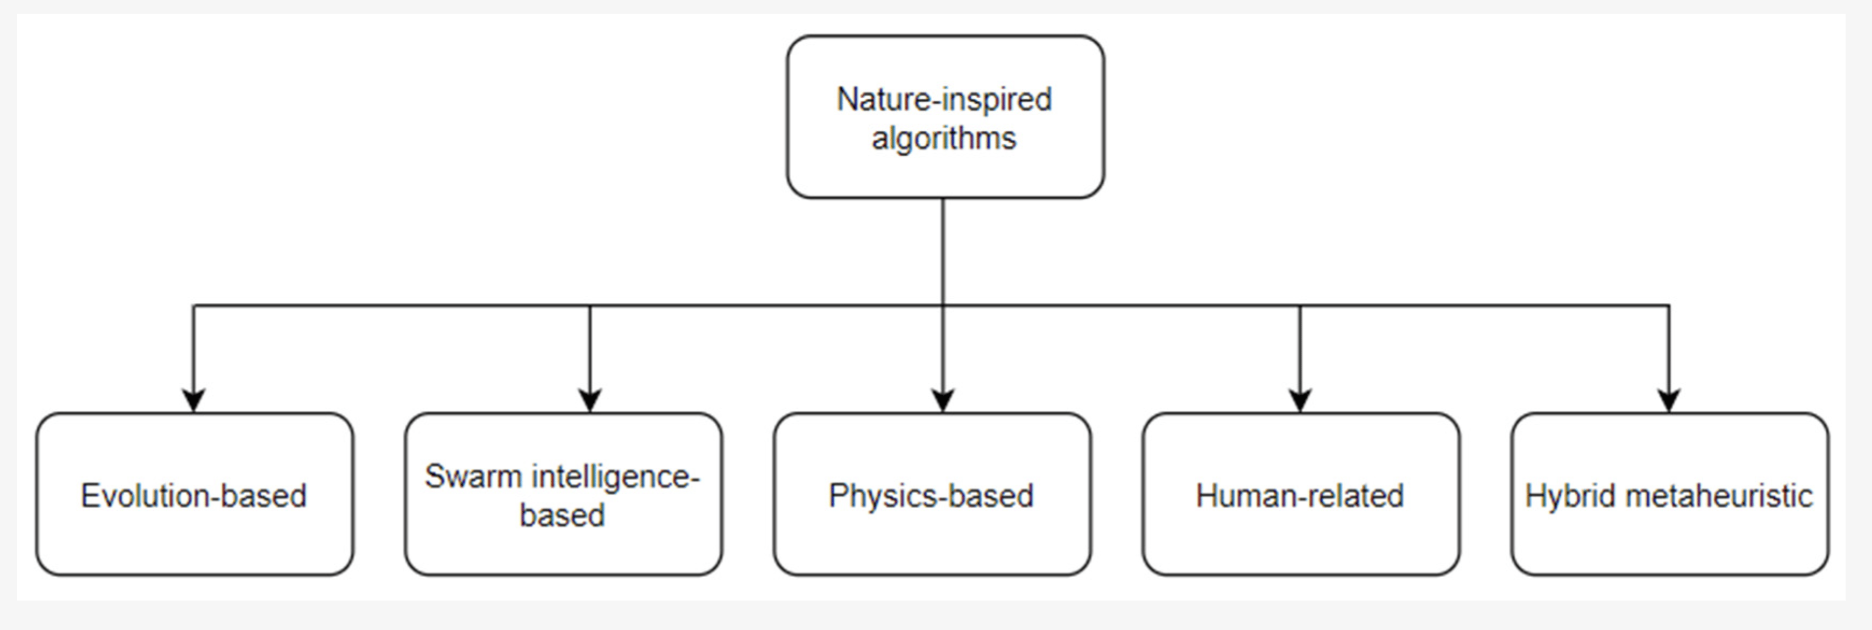
\includegraphics[width=0.9\textwidth]{classification_2.png}
\end{frame}

\begin{frame}{Antecedentes}
    \begin{itemize}
        \item Algoritmos inspirados en humanos 
    \end{itemize}
    \vspace{0.5cm}
    \centering
    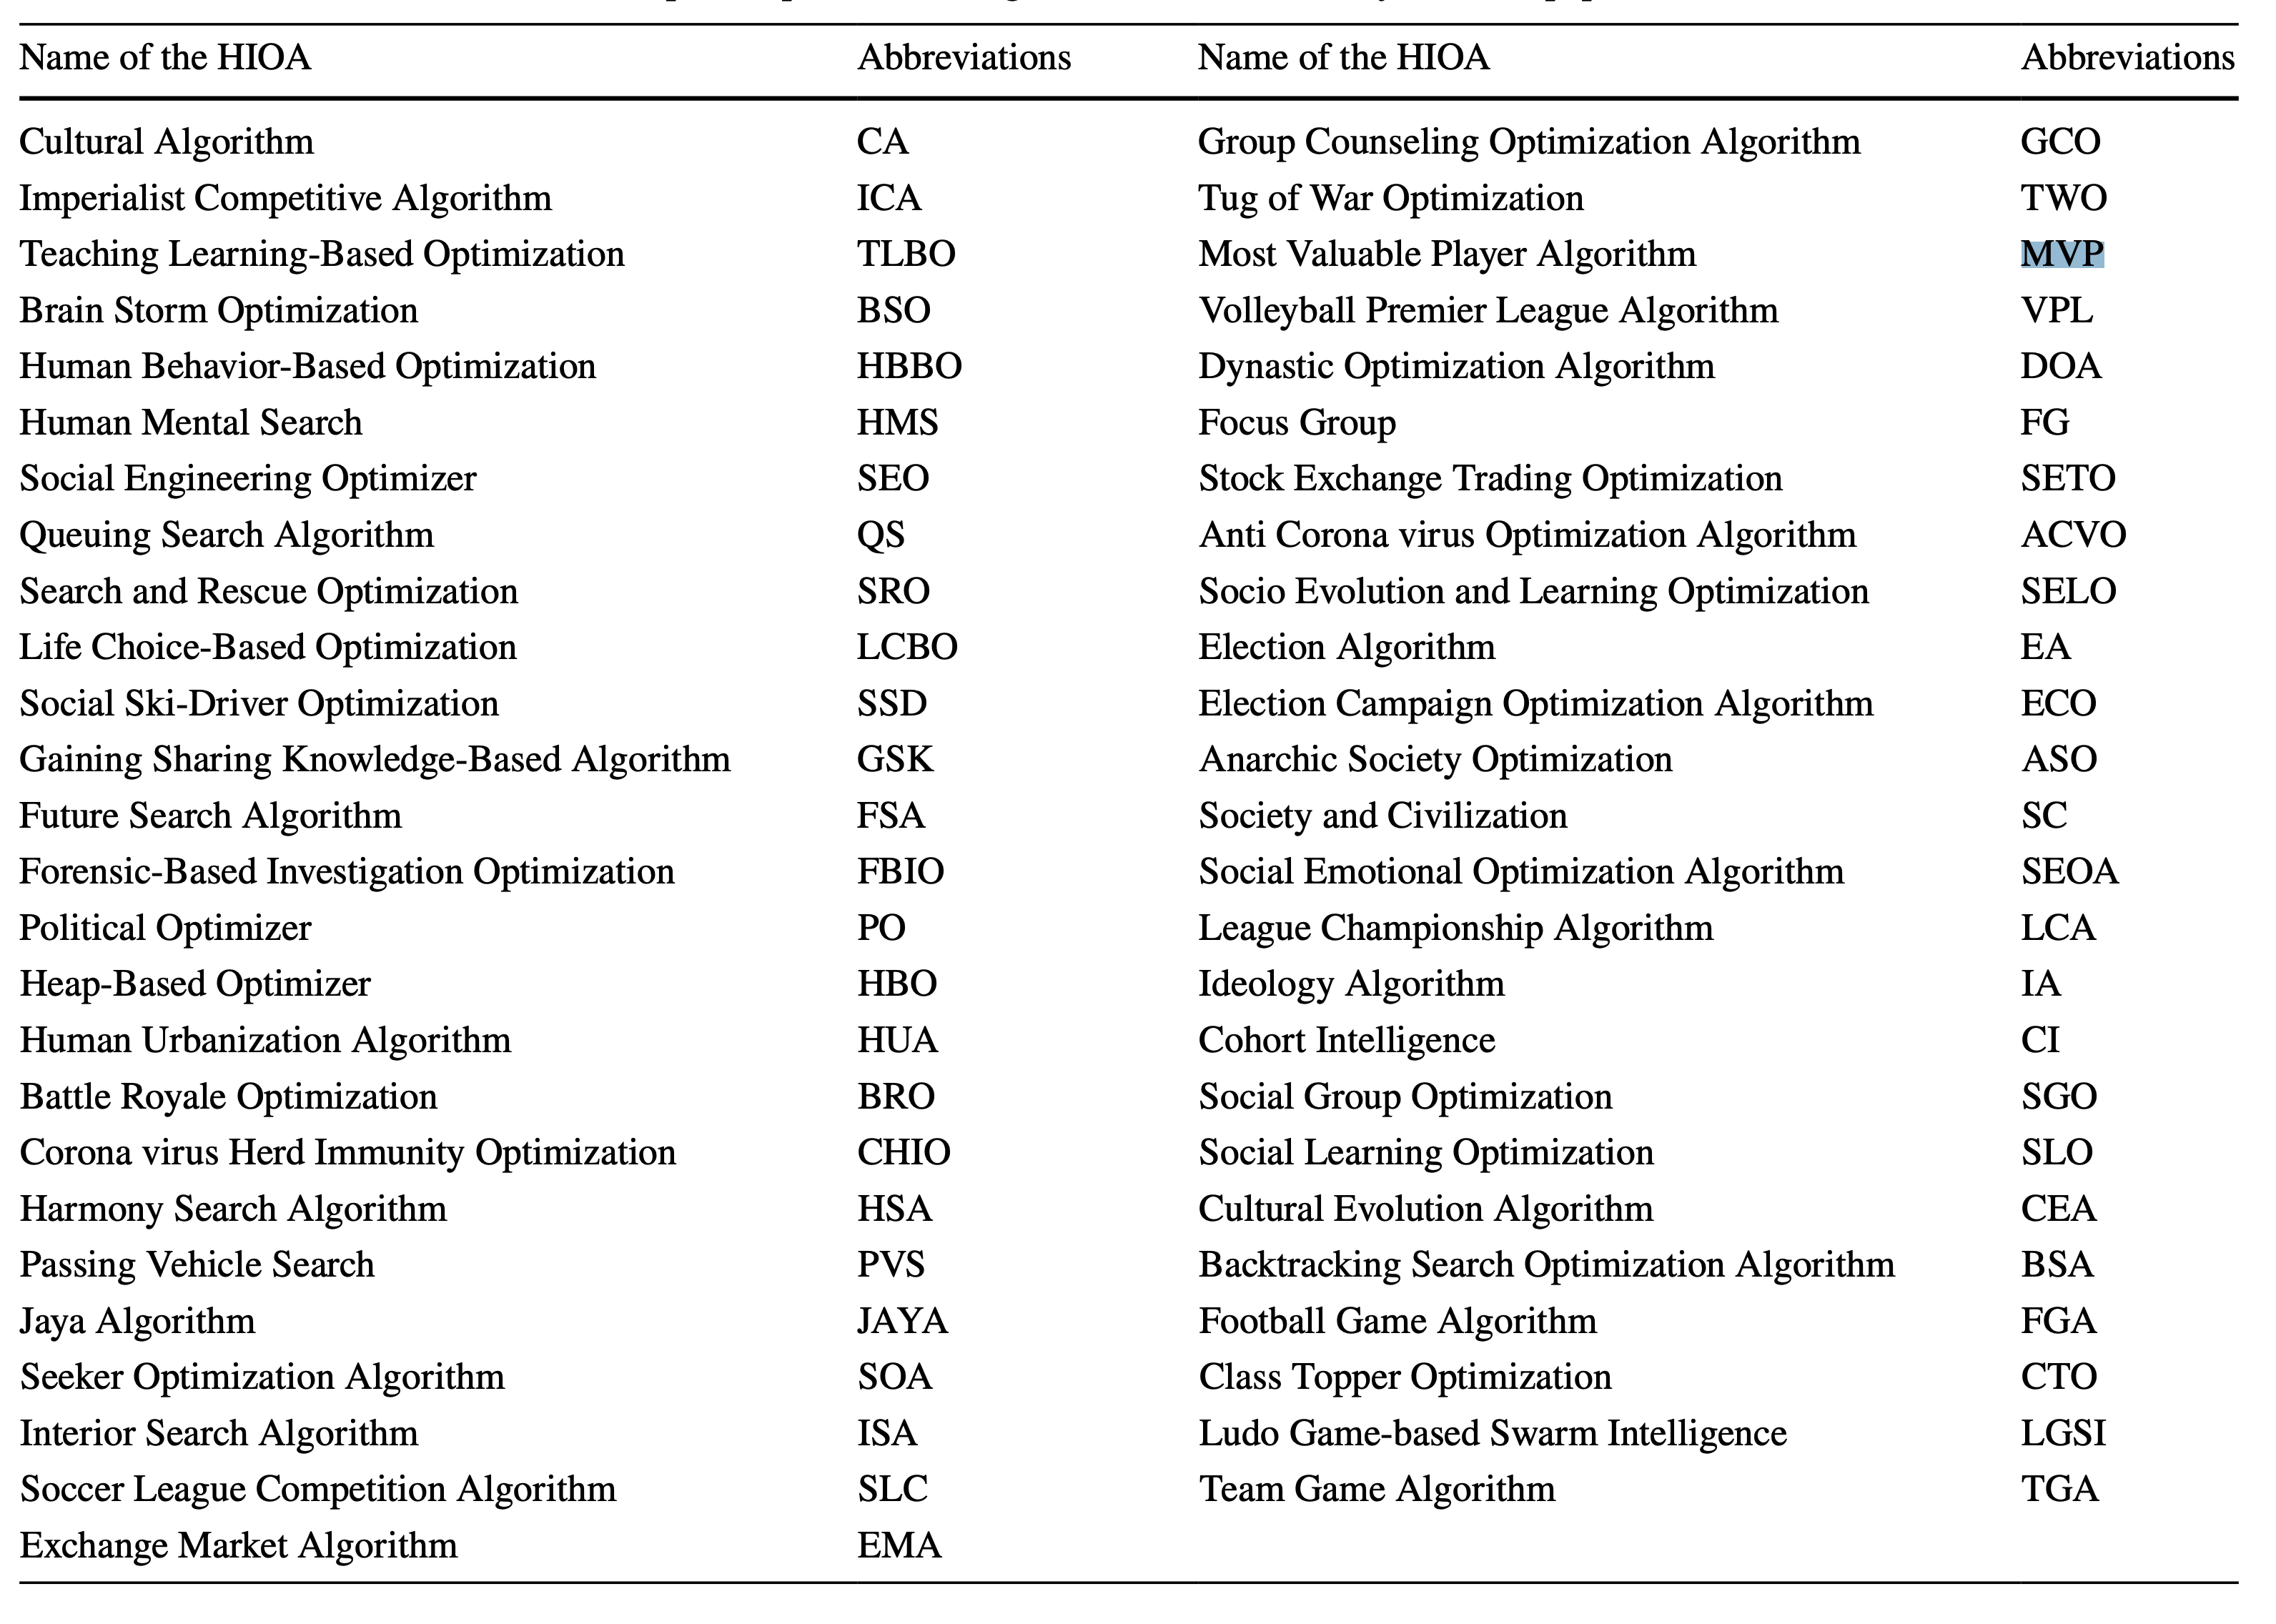
\includegraphics[width=0.9\textwidth]{human-inspired-list.png}
\end{frame}

\begin{frame}{Antecedentes}
    \begin{itemize}
        \item Clasificación de los algoritmos inspirados en humanos 
    \end{itemize}
    \vspace{0.5cm}
    \centering
    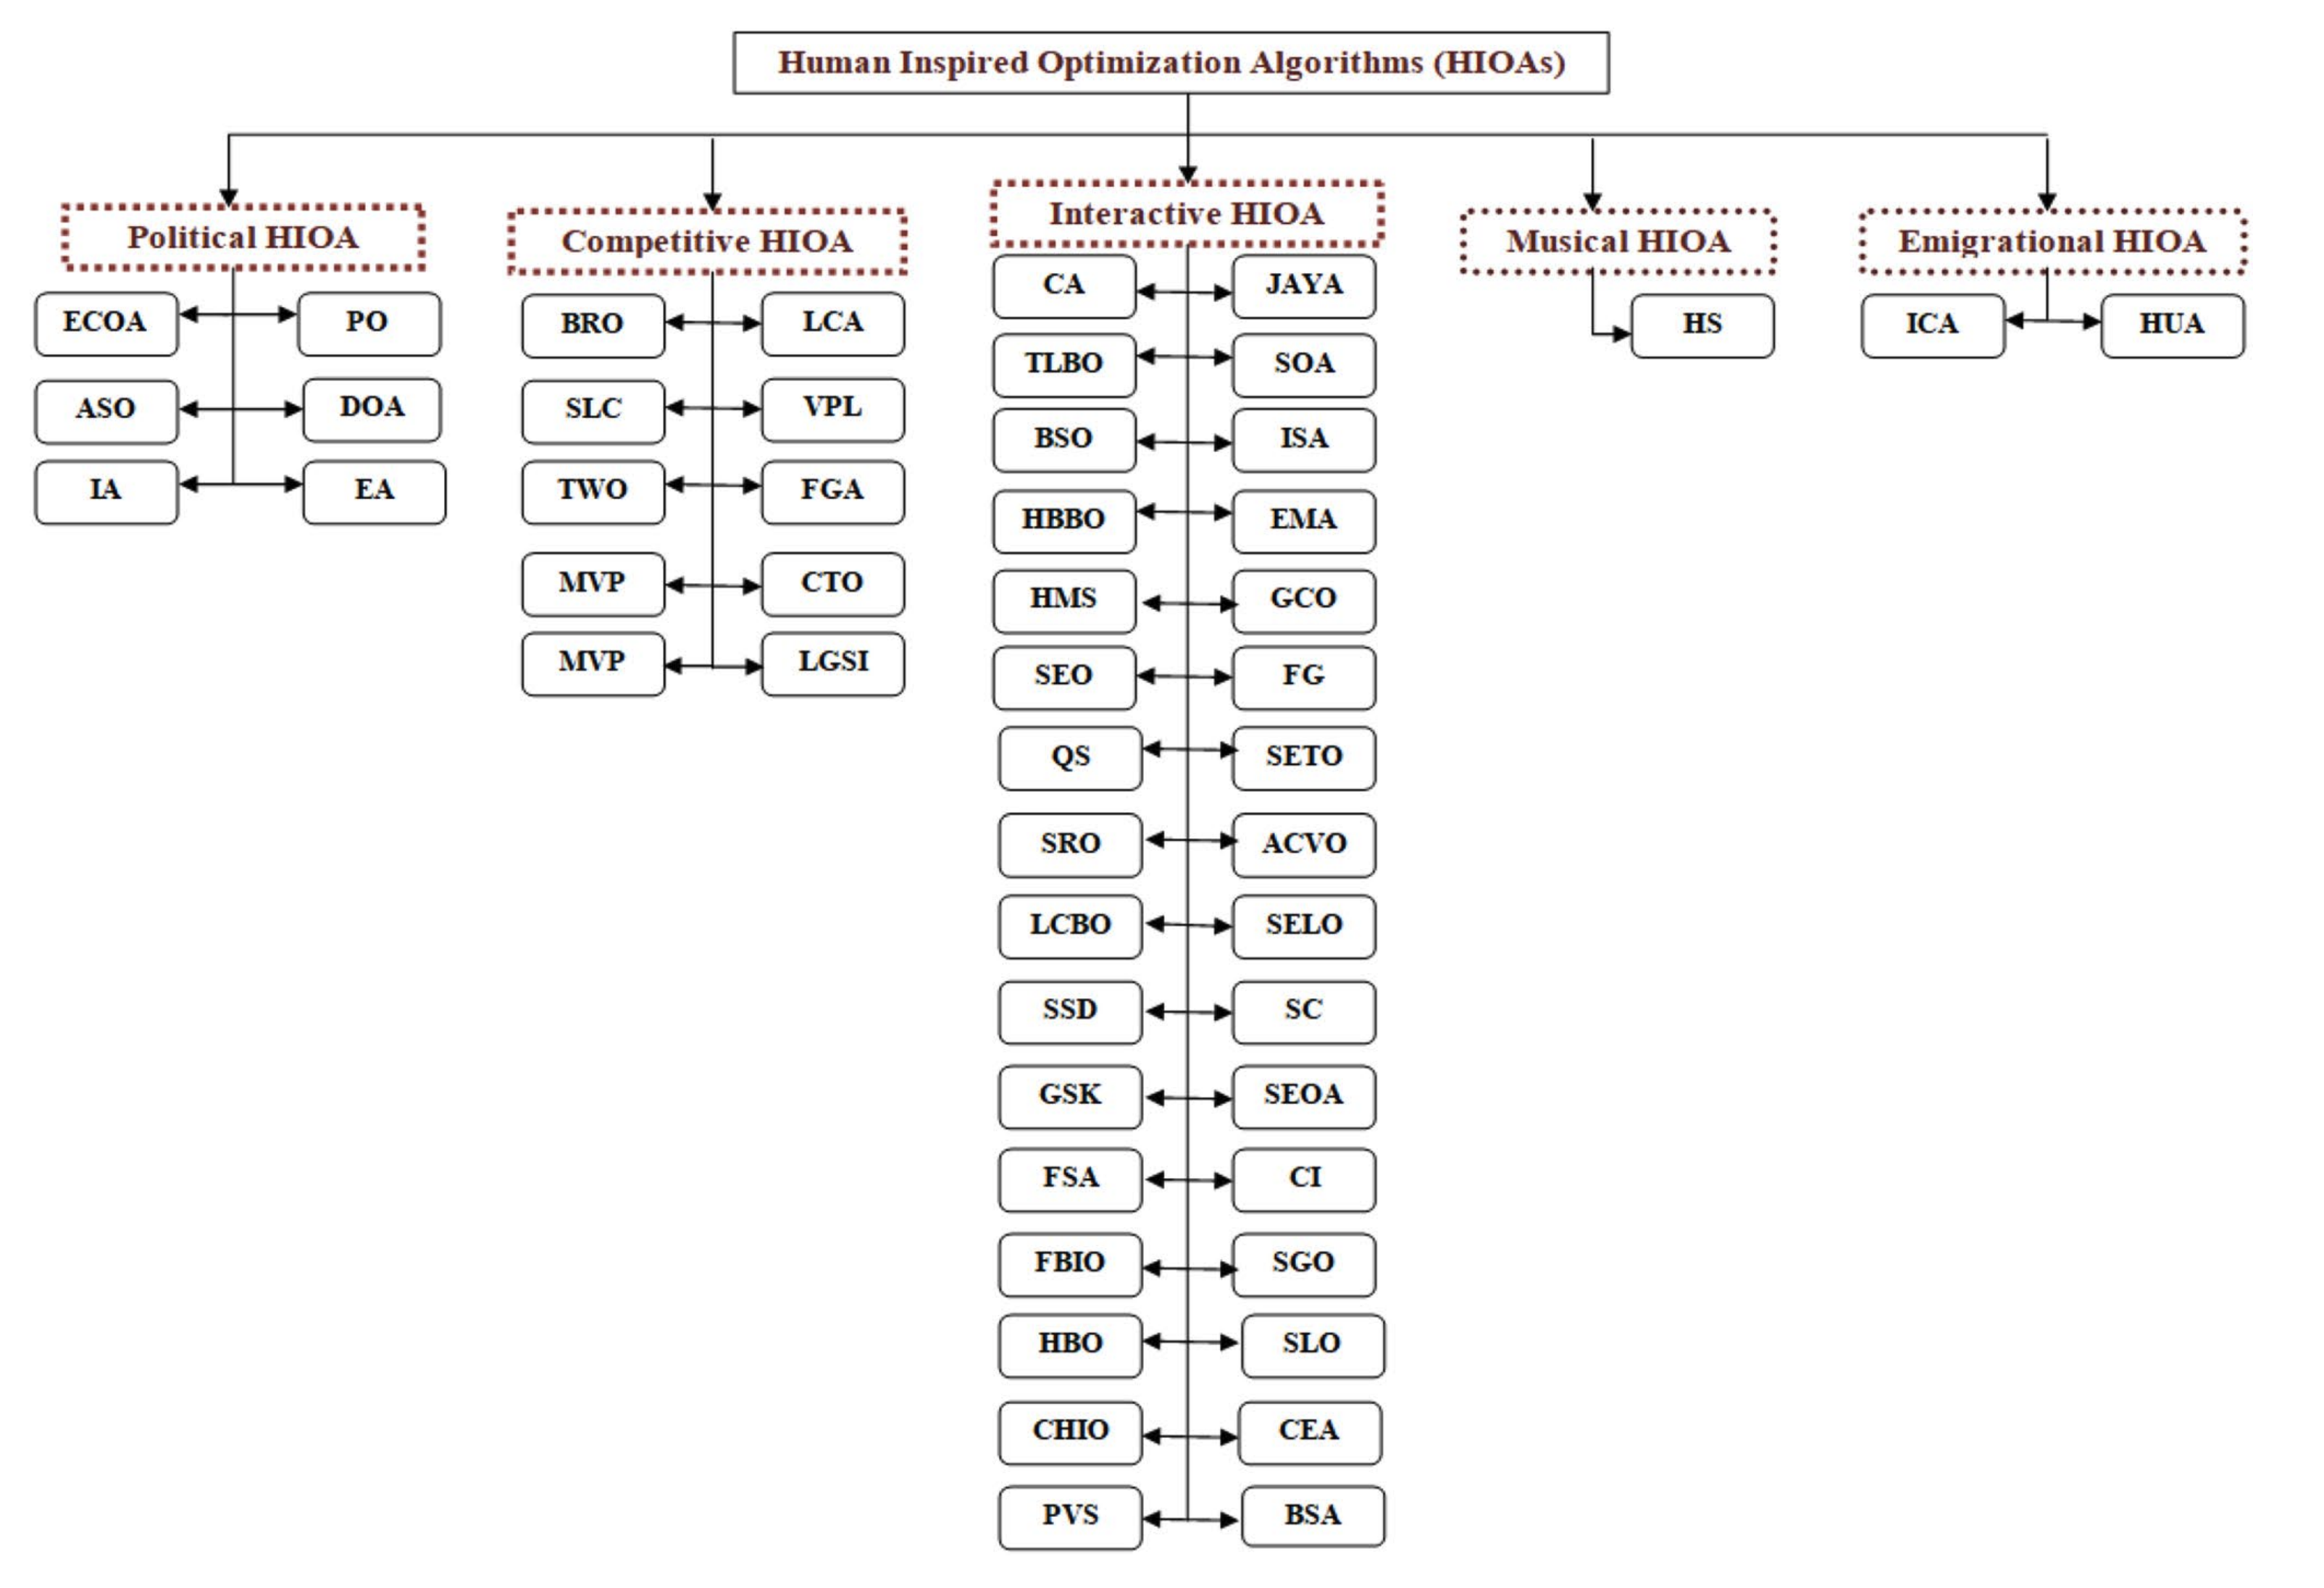
\includegraphics[width=0.9\textwidth]{human-inspired-class.png}
\end{frame}



\section{Introducción}


\begin{frame}{Algoritmos Sociales}
    \begin{itemize}
        \item Dado los antecedentes, entonces podemos hablar del grupo de algoritmos inspirados en fenómenos sociales. 
        \item Debido a la cantidad de algoritmos "existentes", se presentan estrategias generales propias de este grupo de algoritmos.
        \vspace{1cm}
        \begin{itemize}
            \item Liderazgo
            \item Formación de alianzas
            \item Etiquetas sociales
            \item Segregación de vecinos/vecindarios
            \item \textit{Interacciones culturales*} 
        \end{itemize}
    \end{itemize}
\end{frame}

\begin{frame}{Estudio de los fenómenos sociales (Humanos)}
\begin{itemize}
    \item El estudio de los fenómenos sociales se ha dictado por la influencia \textbf{cultural} de las civilización en cada época.
    \item La teoría de sistemas complejos, establece que el comportamiento de un sistema no es viable mediante el estudio de sus componentes por separado, en su lugar, es necesario definir la relación que existe entre sus componentes. (No lineares + Conflictos)

    \item Estos hechos, abren una comunicación bidireccional entre el estudio de los fenómenos sociales y su aplicación a los sistemas computacionales.
\end{itemize}
\end{frame}

\begin{frame}{Estudio de los fenómenos sociales (Humanos)}
\begin{itemize}
    \item Se da por entendido, que en el estudio de los algoritmos sociales, los \textit{agentes} involucrados pueden no conocer (en la mayoría de los casos) el estado de los demás \textit{agentes}.
    \item La sociedad humana (y los algoritmos inspirados en sus fenómenos) tienen la capacidad de \textbf{aprendizaje vicario} (Selección de un modelo, aprendizaje mediante observación mediante la busqueda de información en su vecindario)
    \item Hipótesis: La complejidad de los fenómenos sociales contienen \textit{poder computacional}
\end{itemize}
\end{frame}

\section{Liderazgo}
\begin{frame}{Liderazgo}
    \begin{itemize}
        \item El liderazgo ha sido un fenómeno clave en la organización y evolución de las sociedades humanas.
        \item Inspirado en este fenómeno, se han desarrollado algoritmos de optimización que emulan la influencia de líderes sobre sus seguidores.
        \item Un ejemplo es el \textbf{Society Civilization Algorithm (SCA)}, que explora el espacio de búsqueda utilizando líderes y migración. (Comparación con PSO)
    \end{itemize}
\end{frame}


\begin{frame}{Society Civilization Algorithm (SCA)}
    \textbf{Idea principal del agoritmo:} 
    \begin{itemize}
        \item Los líderes influyen en los individuos de sus sociedades.
        \item La migración y la cooperación son clave para la optimización.
    \end{itemize}
    
    \textbf{Aplicaciones:}
    \begin{itemize}
        \item Optimización de despacho económico en sistemas eléctricos.
        \item Reducción de colisiones en algoritmos de enjambre.
        \item Análisis de datos cuando se requiere hacer agrupación por jerarquías (Clusterización).
    \end{itemize}
\end{frame}

\begin{frame}{Algoritmo General del SCA}
    \begin{enumerate}
        \item Inicializar \( t \leftarrow 0 \).
        \item Generar una \textbf{civilización} \( C(t) \) de \( N \) individuos distribuidos uniformemente.
        \item Evaluar individuos calculando la función objetivo y restricciones.
        \item Construir sociedades \( S(t) \) como \textbf{clusters} usando técnicas de análisis de agrupación.
        \item Identificar líderes en cada sociedad.
        \item Migrar individuos hacia los líderes de sus respectivas sociedades.
        \item Identificar líderes globales en la civilización \( C(t) \).
        \item Migrar líderes de sociedad hacia los líderes globales.
        \item Incrementar \( t \) y repetir hasta cumplir las condiciones de parada.
    \end{enumerate}
\end{frame}

\begin{frame}{Características del SCA}
    \textbf{Elementos clave:}
    \begin{itemize}
        \item \textbf{Migración:} Los individuos se mueven hacia sus líderes locales o globales.
        \item \textbf{Cooperación:} Los líderes comparten conocimiento (posición en el espacio de búsqueda).
        \item \textbf{Exploración y explotación:} Se logran mediante la dinámica de liderazgo y migración.
    \end{itemize}
    
    \textbf{Ventaja principal:}
    \begin{itemize}
        \item Capacidad de evitar mínimos locales.
    \end{itemize}
\end{frame}

\begin{frame}{Otros escenarios relacionados al liderazgo}
\begin{itemize}
    \item Liderazgo es posible ser visto como una influencia Cultural, o agregar el conocimiento de los líderes a un espacio de creencias.
    \item Aproximación de sociedades sin lideres (Anarquismo)
\end{itemize}
\end{frame}

\section{Formación de alianzas}

\begin{frame}{Formación de alianzas}
    \begin{itemize}
        \item La formación de alianzas es un fenómeno social clave en diversos contextos, desde la política hasta los sistemas multiagente.
        \item Este fenómeno se basa en la cooperación y la agrupación para alcanzar objetivos comunes.
        \item En el ámbito de los algoritmos, la formación de alianzas es una inspiración para resolver problemas de optimización que involucran agentes con intereses individuales y colectivos.
    \end{itemize}
\end{frame}

\begin{frame}{Definición de Alianzas}
    \begin{itemize}
        \item Una \textbf{alianza} es un grupo relativamente estable de agentes que trabajan hacia un objetivo común.
        \item Se forman cuando los agentes encuentran beneficios individuales al colaborar, superando las ganancias que obtendrían de forma independiente.
        \item Ejemplo:
        \begin{itemize}
            \item Coaliciones políticas en sistemas multipartidistas.
        \end{itemize}

    \item (Teoría de juegos y el dilema del prisionero)
    \end{itemize}
\end{frame}

\begin{frame}{Características de las Alianzas}
    \begin{itemize}
        \item \textbf{Estabilidad:} Una alianza es estable si sus miembros prefieren mantenerse en ella antes que unirse a otra.
        \item \textbf{Ruptura:} Al alcanzar un tiempo crítico, las alianzas pueden reconfigurarse o disolverse.
        \item \textbf{Comunicación limitada:} En la mayoría de los escenarios, los agentes tienen información incompleta sobre los demás.
    \end{itemize}
    
    \textbf{Problema de optimización:}
    \[
    C = \text{minarg} \sum_{i,k} \delta (A_i, A_k)
    \]
    donde \( \delta(A_i, A_k) \) mide la diferencia entre agentes en términos de sus características y preferencias.
\end{frame}

\begin{frame}{Ejemplo de alianzas es un espacio de partidos políticos}
    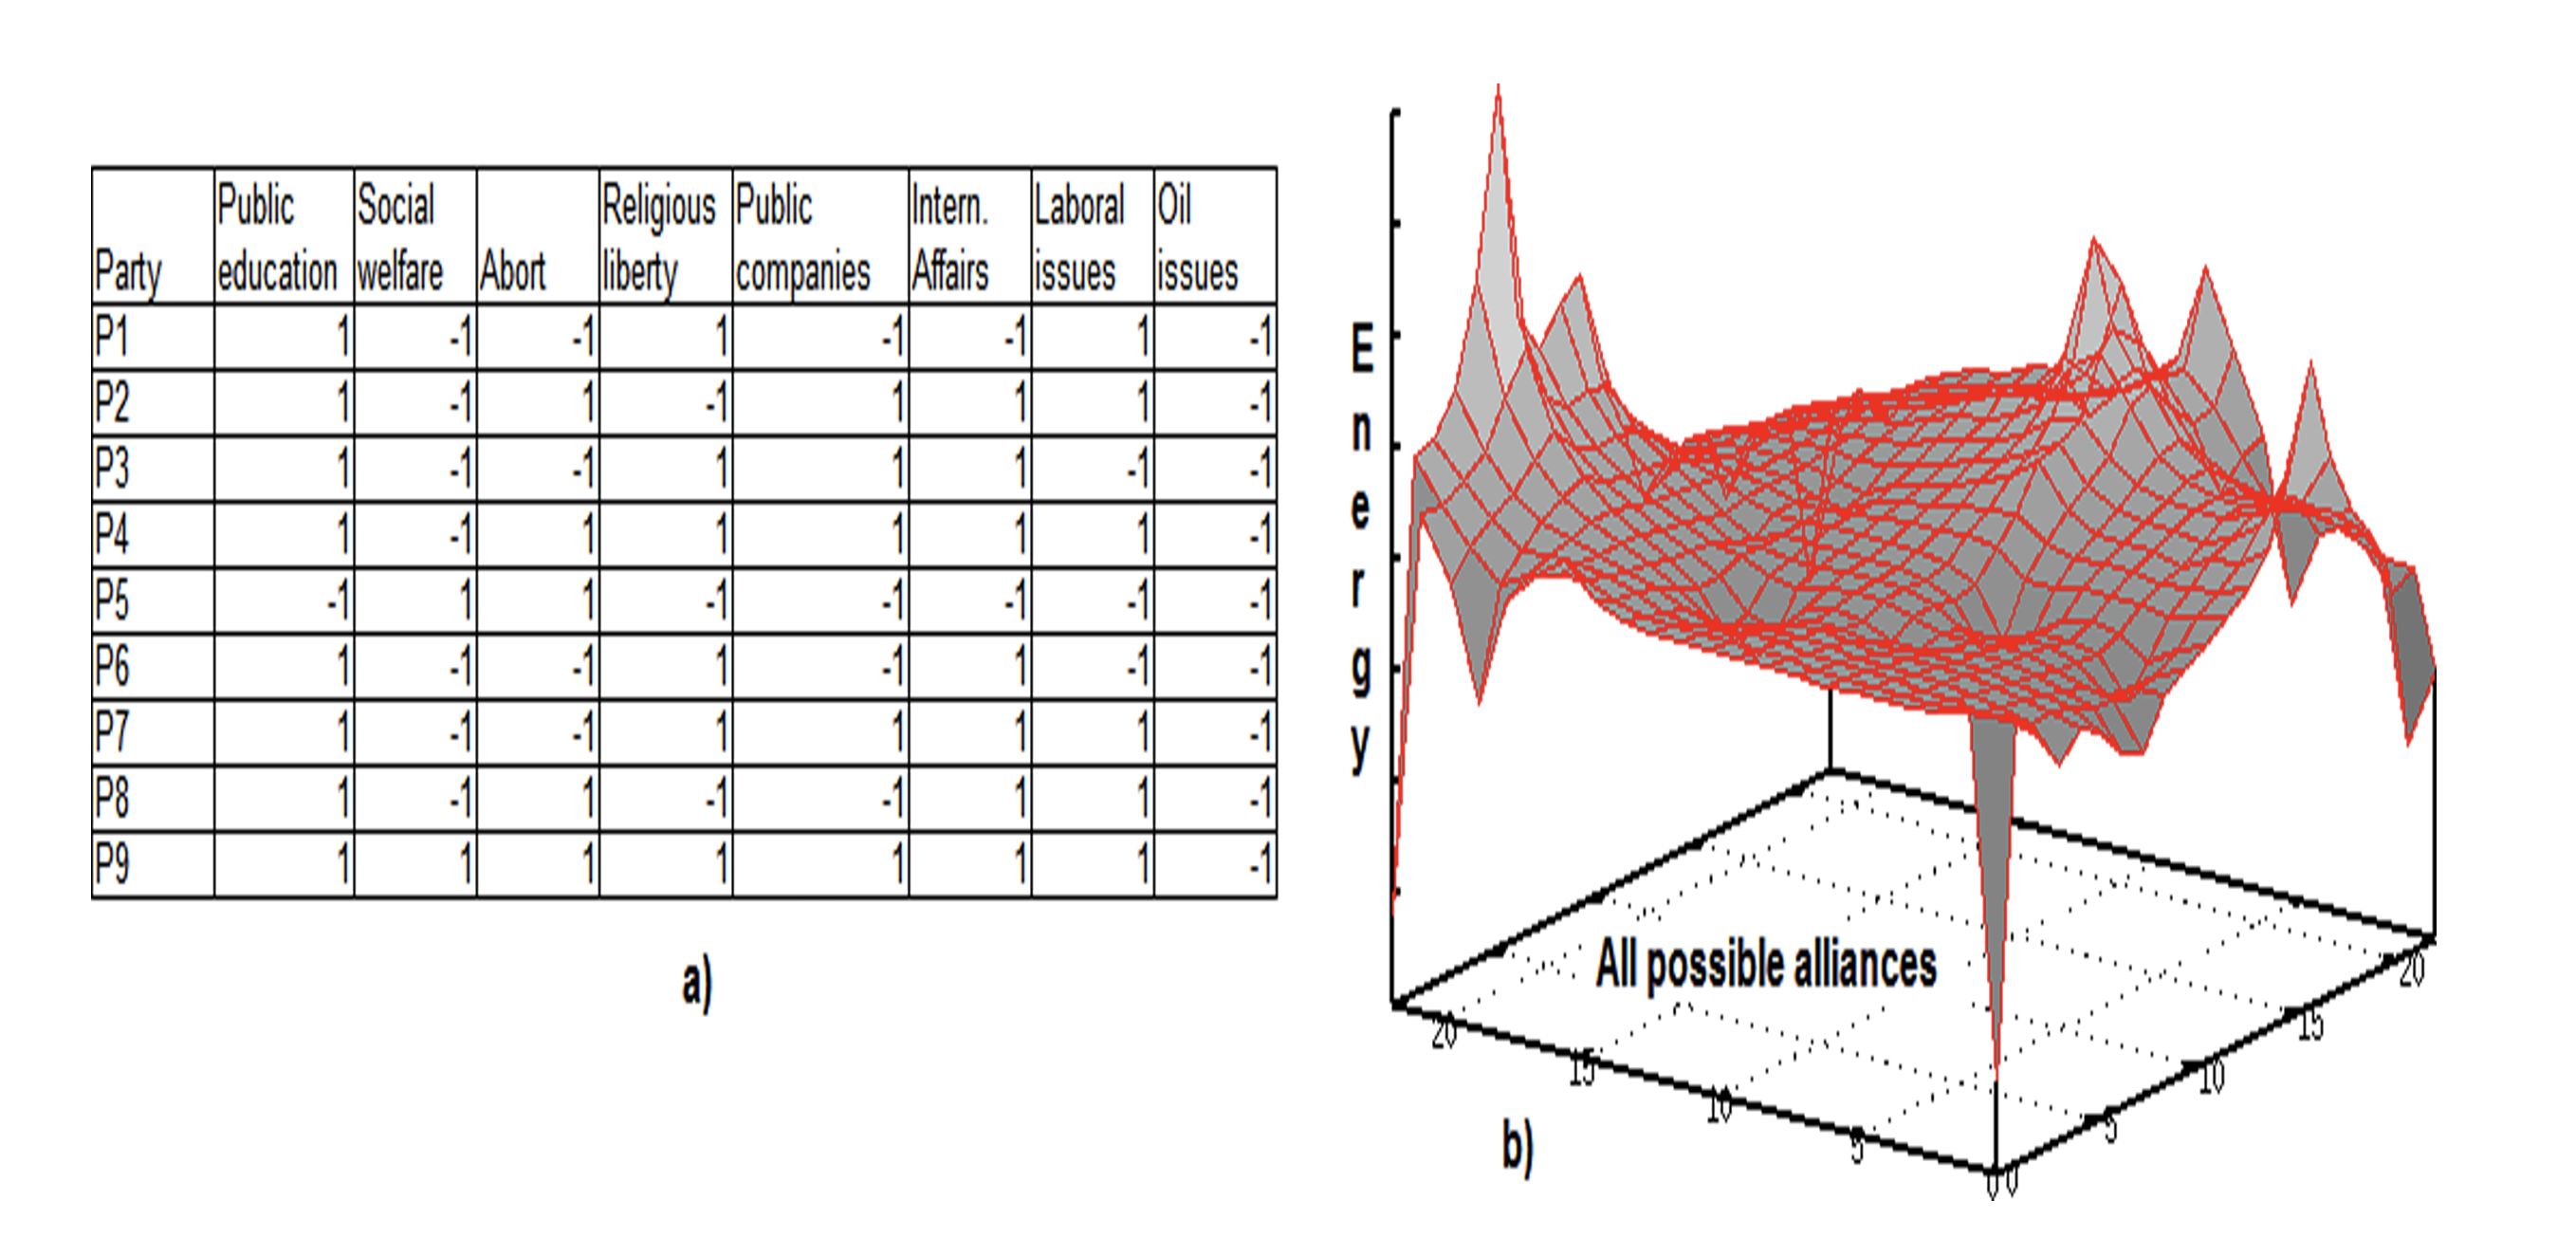
\includegraphics[width=1\textwidth]{alianzas.png}
    La estabilidad de las alianzas se miden por el nivel de energía presente (a mayores similitudes en los intereses, menor energía, mayor estabilidad)
\end{frame}

\begin{frame}{Algoritmo de Formación de Alianzas}
    \textbf{Pasos principales:}
    \begin{enumerate}
        \item Construir una lista de posibles alianzas \( S_i(q) \) con hasta \( q \) agentes.
        \item Mientras \( S_i(q) \) no esté vacío:
        \begin{enumerate}
            \item Contactar agentes \( A_j \in S_i(q) \).
            \item Evaluar el beneficio de unirse a la alianza, sujeto a preferencias y restricciones.
            \item Compartir subtareas con los agentes de la alianza.
        \end{enumerate}
        \item Actualizar las alianzas según los beneficios evaluados.
    \end{enumerate}
\end{frame}

\begin{frame}{Aplicaciones}
    \begin{itemize}
        \item \textbf{Sistemas multiagente:} Resolución de tareas mediante la formación de coaliciones.
        \item \textbf{Política:} Simulación de coaliciones políticas en contextos multipartidistas.
        \item \textbf{Negocios:} Alianzas estratégicas entre empresas para maximizar beneficios compartidos.
    \end{itemize}
    
    \textbf{Ejemplo destacado:}
    \begin{itemize}
        \item Modelo de Axelrod sobre la formación de alianzas durante la Segunda Guerra Mundial, basado en diferencias de características entre agentes. (Autómatas celulares)
    \end{itemize}
\end{frame}

\section{Etiquetado social}
\begin{frame}{Etiquetado social}
    \begin{itemize}
        \item El etiquetado social (\textit{social labeling}) es un fenómeno común en las sociedades humanas.
        \item Las etiquetas asignadas a los individuos pueden influir en cómo otros interactúan con ellos.
        \item Este concepto ha inspirado algoritmos para fomentar cooperación, clasificación y optimización en sistemas distribuidos.
    \end{itemize}
\end{frame}

\begin{frame}{Concepto de Etiquetado Social}
    \begin{itemize}
        \item Una etiqueta o \textit{tag} representa características sociales asignadas a un individuo.
        \item Puede inducir reacciones positivas o negativas en interacciones.
        \item Ejemplos:
        \begin{itemize}
            \item Clasificación de individuos en grupos cooperativos o no cooperativos.
            \item Asignación de etiquetas en redes \textit{Peer-to-Peer} (P2P) para optimizar interacciones.
        \end{itemize}
    \end{itemize}
\end{frame}

\begin{frame}{Optimización en Redes P2P}
    \textbf{Ejemplo: Mejora de cooperación en redes P2P}
    \begin{itemize}
        \item Los nodos son etiquetados como cooperativos o no cooperativos.
        \item Algoritmo:
        \begin{enumerate}
            \item Seleccionar un compañero de juego \( j \) con una etiqueta similar.
            \item Interactuar usando estrategias basadas en el dilema del prisionero.
            \item Reproducir nodos proporcionalmente a sus beneficios.
            \item Mutar etiquetas y estrategias para nodos reproducidos.
        \end{enumerate}
        \item Resultado: Minimización de intentos para obtener recursos deseados.
    \end{itemize}
\end{frame}

\begin{frame}{Algoritmo de etiquetado social}
    \begin{enumerate}
        \item Mientras el número de generaciones no se haya alcanzado:
        \begin{enumerate}
            \item Para cada agente \( i \) en la población:
            \begin{itemize}
                \item Seleccionar un agente \( j \) con una etiqueta similar.
                \item Interactuar mediante estrategias y calcular el beneficio obtenido.
            \end{itemize}
            \item Reproducir agentes proporcionalmente a su beneficio.
            \item Mutar etiquetas y estrategias de agentes reproducidos.
        \end{enumerate}
    \end{enumerate}
    \textbf{Resultado:} Una red cooperativa eficiente, con interacciones optimizadas mediante etiquetas.
\end{frame}

\begin{frame}{Ventajas}
    \begin{itemize}
        \item \textbf{Eficiencia:} Reducción del número de intentos para alcanzar objetivos cooperativos.
        \item \textbf{Clasificación:} Separación efectiva entre agentes cooperativos y no cooperativos.
        \item \textbf{Adaptabilidad:} Las etiquetas evolucionan dinámicamente para reflejar comportamientos cambiantes.
    \end{itemize}
\end{frame}

\section{Delimitación y segregación de vecinos}

\begin{frame}{Delimitación y segregación de vecinos}
\begin{itemize}
        \item La delimitación de vecindarios y la segregación son fenómenos comunes en sociedades humanas.
        \item Estos procesos son resultado de decisiones individuales influenciadas por preferencias económicas, políticas y sociales.
        \item Este comportamiento ha inspirado algoritmos utilizados en urbanismo, análisis de redes y optimización.
    \end{itemize}
\end{frame}

\begin{frame}{Definición del Problema}
    \begin{itemize}
        \item Cada agente (\textit{householder}) tiene un conjunto de características que lo describen.
        \item Los agentes buscan vecindarios donde los vecinos sean similares en función de un umbral de satisfacción.
        \item Cuando los agentes no están satisfechos, migran a nuevas ubicaciones, resultando en segregación.
    \end{itemize}
    
    \textbf{Ejemplo:} Modelo de Schelling (SM) de segregación:
    \begin{itemize}
        \item Agentes en una cuadrícula buscan ubicaciones donde estén rodeados por vecinos similares.
        \item La distribución inicial aleatoria evoluciona hacia una estructura segregada.
    \end{itemize}
\end{frame}

\section{Modelo de Schelling (SM)}

\begin{frame}{Modelo de Schelling: Algoritmo}
    \textbf{Pasos principales:}
    \begin{enumerate}
        \item Cada agente calcula la fracción de vecinos similares \( F_i \).
        \item Si \( F_i > T_i \) (umbral de satisfacción), el agente permanece en su ubicación.
        \item Si \( F_i \leq T_i \), el agente busca la ubicación más cercana que cumpla con el umbral y se muda.
    \end{enumerate}
    \textbf{Resultado:} 
    \begin{itemize}
        \item Segregación espontánea y autoorganización.
        \item Configuraciones estables y estructuradas tras múltiples iteraciones.
    \end{itemize}
\end{frame}

\begin{frame}{Ventajas del Modelo de Schelling}
    \begin{itemize}
        \item \textbf{Simplicidad:} Reglas locales simples producen comportamientos complejos.
        \item \textbf{Adaptabilidad:} Los modelos pueden ajustarse para reflejar características específicas de agentes o redes.
        \item \textbf{Aplicaciones múltiples:} Desde urbanismo hasta redes distribuidas.
        \item \textbf{Autoorganización:} Genera estructuras organizadas sin necesidad de un control central.
    \end{itemize}
\end{frame}

\end{document}